% tex for data

\documentclass{article}
\usepackage{url,graphicx,tabularx,array,amsmath,amssymb,amsthm,booktabs,float}
\usepackage[margin=.65in]{geometry}
\graphicspath{{C:/Users/Colin/Documents/GitHub/533-proj/}{C:\Users}}
\begin{document}
Data:\\\\
The data analyzed is hard drive testing data from the company Backblaze.  Since 2013, Backblaze has been continuously spinning hard drives in controlled storage pods.  When a hard drive fails it is removed from testing, and new hard drives are regularly added to the testing sample.  The latest data provided by Backblaze goes from January 1, 2015 to September 30, 2015.  In addition to providing the time the hard drive failed, the data set has the number of hours a hard drive has been on test, as well as the model and brand of the hard drive.\\
There were initially 54,398 drives in the sample.  Before analyzing the data, however, we removed certain observations.  Any models with fewer than 100 drives in testing were excluded.  Also, drives that failed in fewer than 20 days were removed.  There were some other bizzare observations in the data; for example, hard drives listed as being in test for over 10 years or drives that entered and exited the sample on the same day.  There bizzare observations were likely due to mis-coding and were dropped. After cleaning the data we had a sample size of 52,811 total drives.\\

There were a total of 21 models in the final sample.  Below is a summary of the distribution of failures and total testing time by model.  The total number of failures was 1030.  The majority of those failures were from models 5, 7, 9, and 11.  Not suprisinglu, model 11, which had the most failures also had the longest total testing time; however, this relationship was not uniform across models.  Model 1 had the 2nd longest total testing time, but relatively few failures.
\begin{figure}[H]
\centering
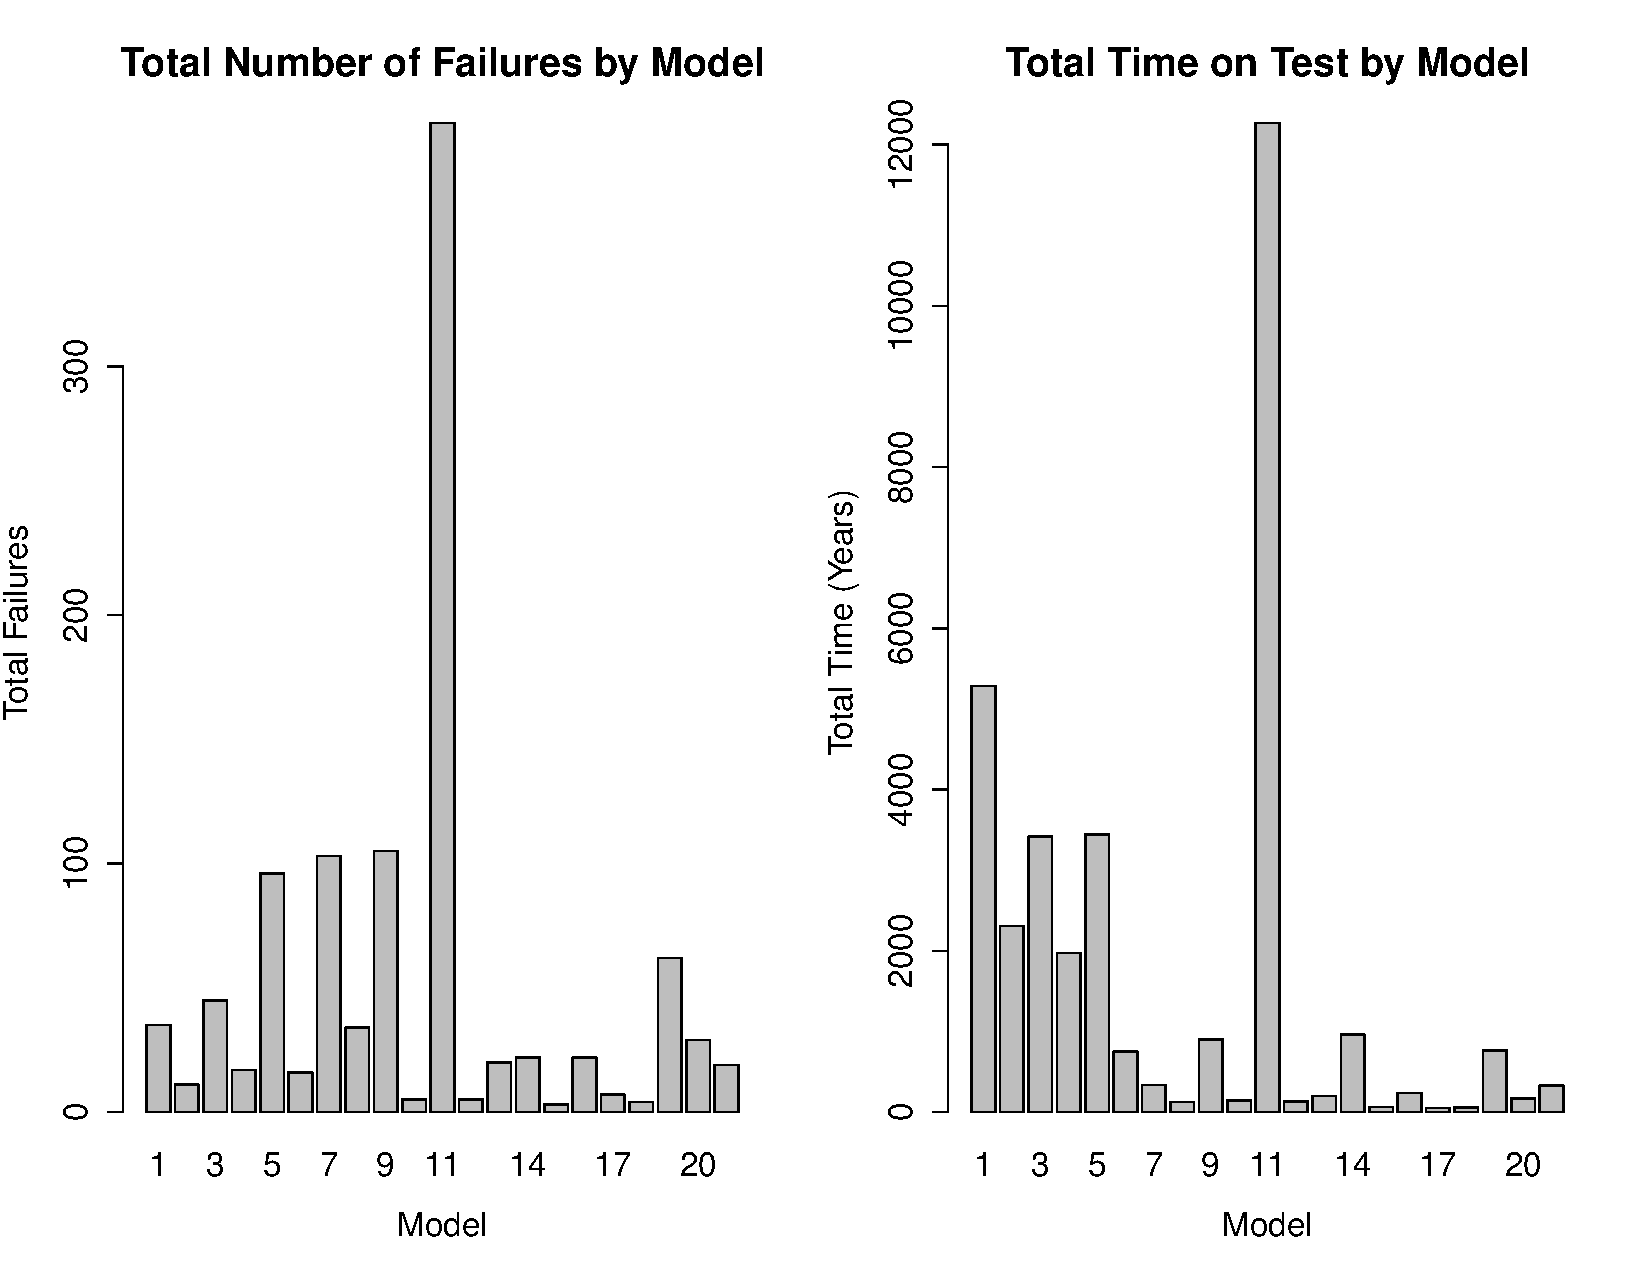
\includegraphics[height=12cm]{sumstat1.pdf}
\end{figure}
We also examined the distribution of failure times.  The shape is slightly skewed to the right with the majority of failures occuring within 250 days.  This might indicate 

\begin{figure}[H]
\centering
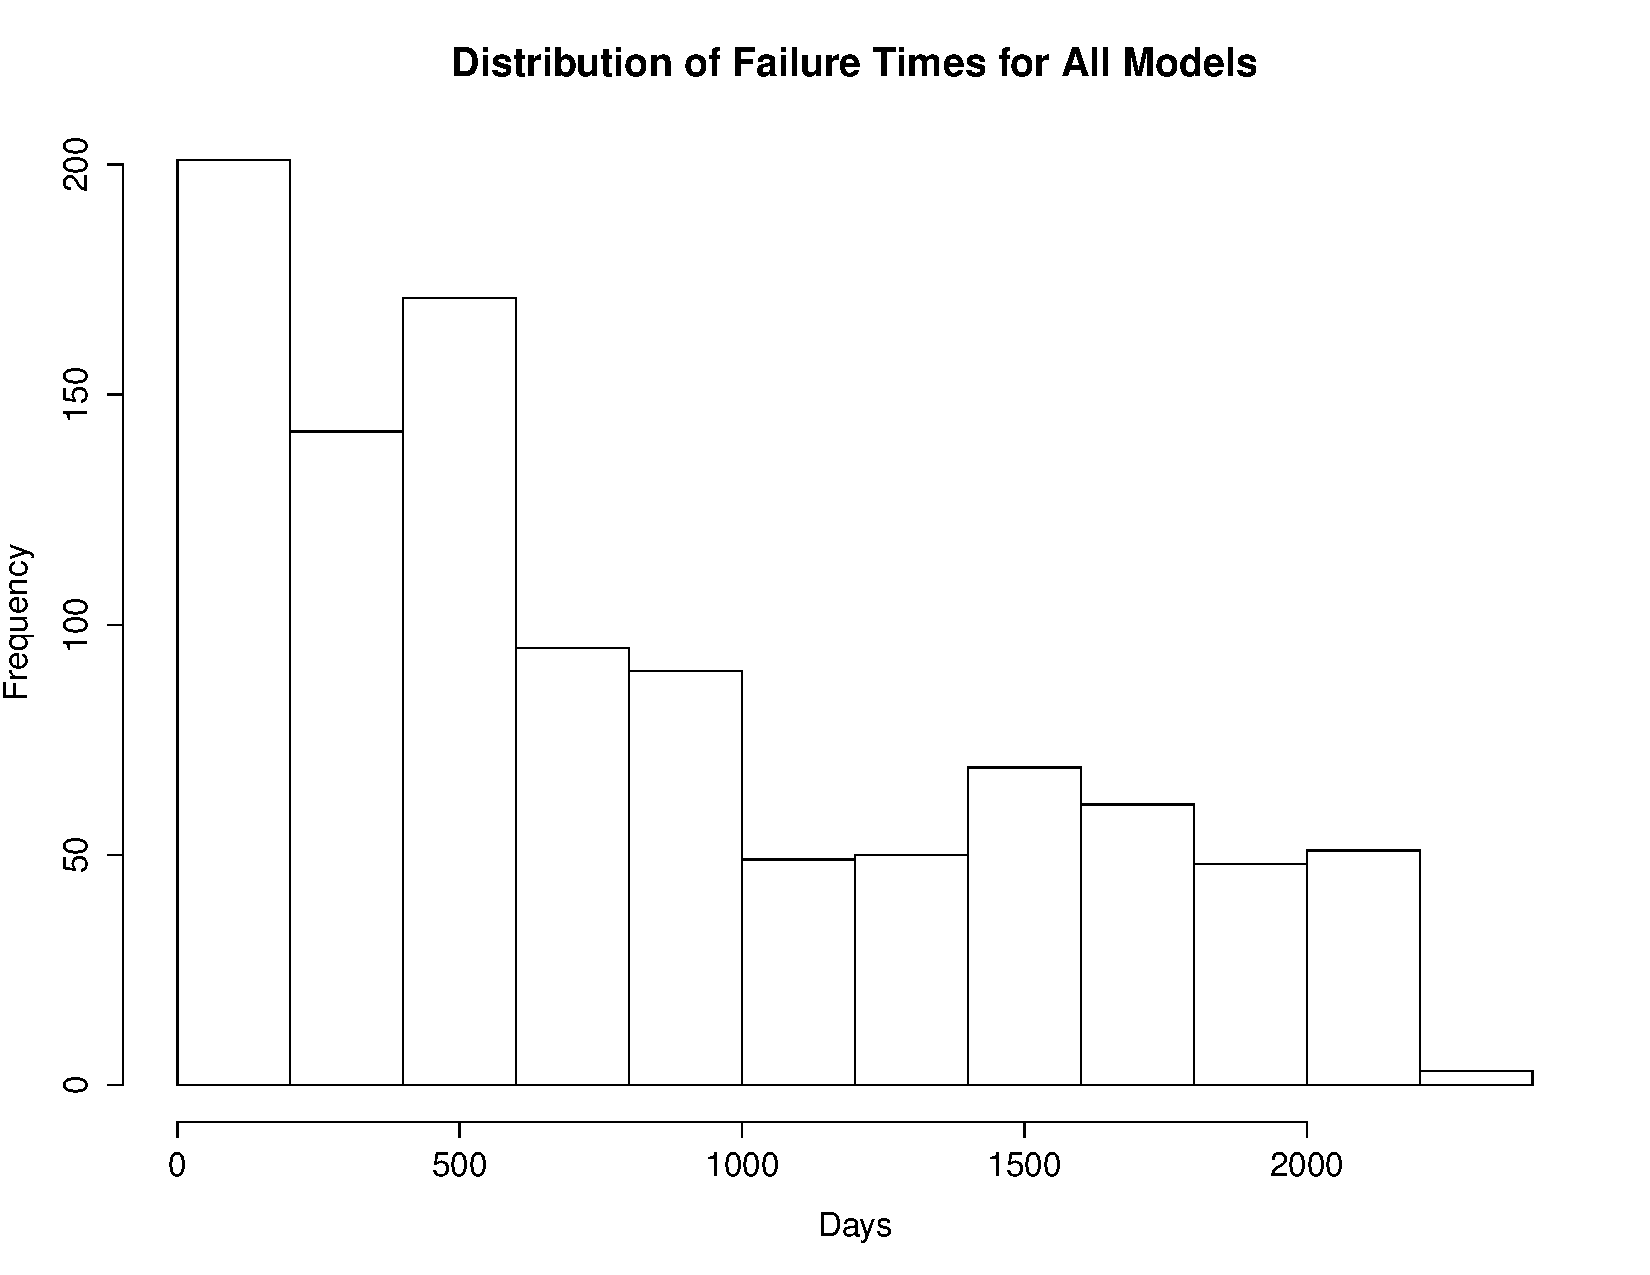
\includegraphics[height=12cm]{sumstat2.pdf}
\end{figure}
\end{document}

